\documentclass[11pt,aspectratio=169]{beamer}
\usepackage[T1]{fontenc}
\usepackage[utf8]{inputenc}
\usepackage[english]{babel}
\usepackage{mathpazo}
\usefonttheme{serif}
\usepackage{amsmath,amssymb,booktabs,array,tabularx,graphicx,microtype}
\usepackage{adjustbox}
\usepackage{tikz}
\usetikzlibrary{arrows.meta,calc,positioning,decorations.pathreplacing,patterns,fit,backgrounds}

% Figures come from the idea folder; the TikZ figures in tikz/ are copies of those of the note.
\graphicspath{{../../ideas/group-identification/figures/}}

% Colours of the note: i, j and a third flight; neutrals for text, grids and fills.
\definecolor{blueI}{HTML}{2A78D6}
\definecolor{orangeJ}{HTML}{EB6834}
\definecolor{aqua}{HTML}{1BAF7A}
\definecolor{ink}{HTML}{0B0B0B}
\definecolor{ink2}{HTML}{52514E}
\definecolor{muted}{HTML}{9A9893}
\definecolor{light}{HTML}{E6E5E1}
\definecolor{steel}{RGB}{74,96,121}
\definecolor{steellight}{RGB}{192,206,220}

\tikzset{
  >={Stealth[length=1.8mm]},
  every picture/.style={line cap=round, line join=round},
  lbl/.style={font=\footnotesize},
  note/.style={font=\footnotesize, text=ink2},
}

\newcommand{\x}{\mathbf{x}}
\newcommand{\dep}{\mathrm{dep}}
\newcommand{\fin}{\mathrm{fin}}

% Theme: steel-blue title bar, white pages, as in the earlier decks.
\setbeamercolor{structure}{fg=steel}
\setbeamercolor{normal text}{fg=ink,bg=white}
\setbeamercolor{frametitle}{fg=white,bg=steel}
\setbeamercolor{alerted text}{fg=blueI}
\setbeamercolor{takeaway}{fg=steel,bg=steellight!30}
\setbeamercolor{defbox}{fg=ink,bg=steellight!28}
\setbeamersize{text margin left=7mm,text margin right=7mm}
\setbeamertemplate{navigation symbols}{}
\setbeamertemplate{itemize item}{\textcolor{steel}{\small$\bullet$}}
\setbeamertemplate{itemize subitem}{\textcolor{steel}{\textendash}}
\setbeamertemplate{itemize/enumerate body begin}{\setlength{\itemsep}{0.3em}}
\setbeamertemplate{frametitle}{%
  \nointerlineskip
  \begin{beamercolorbox}[wd=\paperwidth,ht=9mm,dp=3mm,center]{frametitle}
    \large\insertframetitle\strut
  \end{beamercolorbox}
  \begin{tikzpicture}[remember picture,overlay]
    \node[anchor=north east,text=white,inner sep=0pt,xshift=-2.3mm,yshift=-4.2mm]
      at(current page.north east){\small\insertframenumber};
  \end{tikzpicture}}
\setbeamertemplate{footline}{%
  \hspace{7mm}\textcolor{muted}{\fontsize{6.5}{8}\selectfont
    Matteo Di Sante\enspace|\enspace Method assessment\enspace|\enspace xc-lab, 23 October 2026}\vspace{2mm}}

\newcommand{\source}[1]{\par\vspace{1mm}{\fontsize{7}{8.3}\selectfont\color{ink2}#1\par}}
\newcommand{\takeaway}[1]{\par\vfill
  \begin{beamercolorbox}[wd=\linewidth,sep=5pt]{takeaway}\small #1\end{beamercolorbox}}
% A definition: its name in bold, then the statement, on a pale band.
\newcommand{\defn}[2]{%
  \begin{beamercolorbox}[wd=\linewidth,sep=5pt]{defbox}\small\textcolor{steel}{\textbf{#1.}}\enspace #2\end{beamercolorbox}}
% A TikZ figure of the note, scaled to fit the given height and the line width.
\newcommand{\tikzfig}[2][0.8\textheight]{%
  \begin{center}\adjustbox{max width=\linewidth,max height=#1}{\input{tikz/#2}}\end{center}}
% A figure of the note at full width, at most the given height.
\newcommand{\fig}[2][0.5\textheight]{%
  \begin{center}\includegraphics[width=\linewidth,height=#1,keepaspectratio]{#2}\end{center}}
% A full-page divider that opens one part of the talk.
\newcommand{\partframe}[2]{%
\begin{frame}[plain,noframenumbering]
\begin{tikzpicture}[remember picture,overlay]
 \fill[steel](current page.south west)rectangle(current page.north east);
 \node[text=white,align=center,text width=.82\paperwidth]at([yshift=4mm]current page.center)
   {{\Large\bfseries #1}\\[3mm]{\normalsize\color{steellight}#2}};
\end{tikzpicture}
\end{frame}}

\hypersetup{pdftitle={Method assessment},pdfauthor={Matteo Di Sante},
  colorlinks=true,urlcolor=blueI,linkcolor=blueI}

\begin{document}

\begin{frame}[plain]
\begin{tikzpicture}[remember picture,overlay]
 \fill[steel](current page.south west)rectangle(current page.north east);
 \fill[steellight](current page.south west)rectangle([yshift=20mm]current page.south east);
 \node[text=white,align=center,text width=.9\paperwidth]at([yshift=8mm]current page.center)
   {{\LARGE\bfseries Is it chance?}\\[4mm]
    {\large Calibrating and tuning the group identification}};
 \node[text=steel,align=center]at([yshift=10mm]current page.south)
   {{\normalsize Matteo Di Sante\quad|\quad xc-lab meeting, 23 October 2026}\\[1.5mm]
    {\footnotesize Method note, sections 7--9: \texttt{xc-lab/ideas/group-identification}}};
\end{tikzpicture}
\end{frame}

\begin{frame}{The question}
\begin{beamercolorbox}[wd=\linewidth,sep=6pt,center]{takeaway}
\large Two pilots who never interact still meet.\\ How long must a contact last before it is not chance?
\end{beamercolorbox}
\bigskip
They take off from the same site, follow the same ridges and valleys, climb in the same house
thermals. So:
\begin{itemize}
  \item build \textbf{chance} from the data: pairs that fly the same routes without synchrony;
  \item keep the contacts that are long enough for chance to be \textbf{one in ten};
  \item check how the result moves with each \textbf{threshold}.
\end{itemize}
\source{Run: 162\,485 cleaned flights of 6\,209 dates of the FFVL archive; profiles on 300 random
dates.}
\end{frame}

\partframe{Part 1: what chance means}{The null model and the minimum duration $\tau^*$}

\begin{frame}{The null model: shift one flight in time}
\defn{Surrogate pair}{Two flights of the same date, takeoffs less than $R_s=10$~km apart; the
copy of $j$ takes off $\vartheta$ after $i$, with $\vartheta$ drawn from the takeoff delays of the
day:
\[
  \x^s_j(t)=\x_j(t+r_{ij}),\qquad r_{ij}=(k^0_j-k^0_i)-\vartheta,\qquad |r_{ij}|\ge2\delta+\Delta .
\]}
\tikzfig[0.27\textheight]{null}
\begin{columns}[T,onlytextwidth]
\column{.48\textwidth}
\small\textbf{Keeps}: route, terrain, date, takeoff delays of the day.
\column{.48\textwidth}
\small\textbf{Destroys}: every correspondence within $\delta$, since $|r_{ij}|>2\delta$.
\end{columns}
\source{Up to 200 pairs per date. Idea from Spiegel et al.\ (2016).}
\end{frame}

\begin{frame}{The shifts are about an hour}
\begin{columns}[c,onlytextwidth]
\column{.55\textwidth}
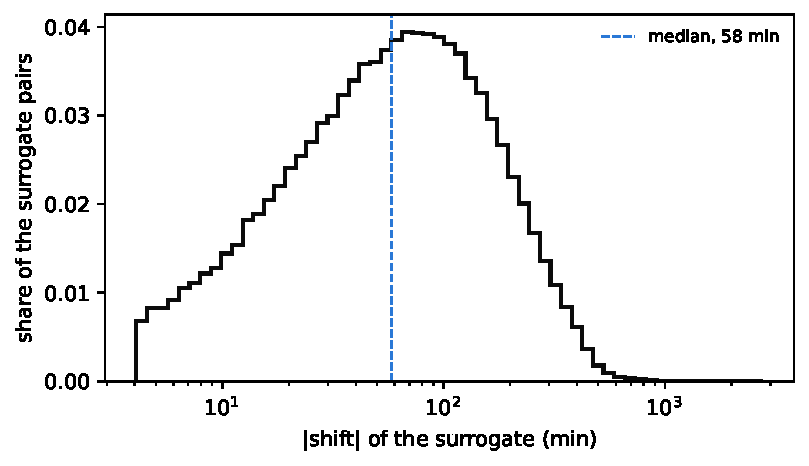
\includegraphics[width=\linewidth]{assessment_shifts.pdf}
\column{.42\textwidth}
\small
Median shift \textbf{58~min}; 90\% between 8~min and 4.4~h.
\par\medskip
The copy flies in the weather of another hour: other thermals, another cloud base.
\par\medskip
So ``real'' includes pilots who share a thermal at the same time without following each other.
\end{columns}
\source{248\,741 surrogate pairs of the chosen run, whole archive.}
\end{frame}

\begin{frame}{From the surrogates to $\tau^*$}
\defn{False discovery rate}{On each date $d$: $H_d$ the exposure of the real pairs (time both fly
after departure), $\rho_{0,d}(\tau)$ the surrogate intervals lasting at least $\tau$ per second
of surrogate exposure. With $N(\tau)$ the real intervals lasting at least $\tau$:
\[
  C(\tau)=\sum_d\rho_{0,d}(\tau)\,H_d,\qquad
  \widehat{\mathrm{FDR}}(\tau)=\frac{C(\tau)}{N(\tau)},\qquad
  \tau^*=\min\bigl\{\tau:\ \widehat{\mathrm{FDR}}(\tau)\le q\bigr\}.
\]}
\medskip
\small
$C(\tau)$: the intervals lasting at least $\tau$ that chance alone would give the real pairs.
\par\smallskip
$\tau^*$: the shortest duration at which chance is at most a share $q$ of what we observe.
\source{The estimate of SAM (Tusher et al.\ 2001), with time shifts in place of permutations;
rates taken date by date because the surrogates are a sample of each date.}
\end{frame}

\begin{frame}{Most short contacts are chance}
\fig[0.5\textheight]{assessment_fdr.pdf}
\source{Left: real intervals lasting at least $\tau$ (solid) and chance (dashed), $\delta=5$~min
(grey) and 2~min (blue). Right: their ratio; dots: $\tau^*$ for $q=0.05$, 0.1, 0.2.}
\takeaway{Chance is 74\% of all pair intervals, 47\% of those lasting 10~min, 16\% of those
lasting 30~min. With $q=0.1$: $\tau^*=38.1$~min (37.0--41.1 over 200 resamplings of the dates).}
\end{frame}

\begin{frame}{How much the shift matters}
\begin{center}
\small
\begin{tabular}{@{}l r c c c c@{}}
\toprule
Surrogates & pairs & $\widehat{\mathrm{FDR}}$(10 min) & $\widehat{\mathrm{FDR}}$(30 min) & $\tau^*$ (min) & 5--95\% \\
\midrule
all shifts & 241\,824 & 0.48 & 0.16 & 38.2 & 37.0--41.5 \\
$|r|<30$ min & 69\,444 & 0.73 & 0.31 & 53.3 & 49.7--72.0 \\
$|r|\ge60$ min & 119\,687 & 0.26 & 0.05 & 23.0 & 21.1--24.4 \\
\bottomrule
\end{tabular}
\end{center}
\source{$q=0.1$, $\delta=2$~min, on the 2\,737 dates with surrogates in each class.}
\medskip
\small
Short shifts keep the weather of the hour, but also bring within $\delta$ the pilots who follow
each other a few minutes apart. The two effects cannot be separated.
\takeaway{The length of the shift moves $\tau^*$ by more than a factor two. We keep the shifts that
follow the takeoff delays of the day.}
\end{frame}

\partframe{Part 2: the parameters on the data}{Measured, chosen, or declared as definitions}

\begin{frame}{Three kinds of parameters}
\begin{center}
\small
\begin{tabularx}{\linewidth}{@{}l l X@{}}
\toprule
Parameter & Value & How it was set \\
\midrule
$\delta$, largest delay & 2 min & measured on the delay profile \\
$q$, accepted false discovery rate & 0.1 & trade-off between groups found and chance \\
$\tau^*$, shortest contact & 38.1 min & computed from $q$ and the null model \\
$\varepsilon_h$, $\varepsilon_z$ & 500 m, 300 m & definitions: profiles without an edge \\
$g$, longest gap joined & 120 s & definition: gaps of real and chance contacts alike \\
$\theta_{\max}$ & 45$^\circ$ & no effect on the result \\
$\Delta$, $h_{\max}$, $R_\dep$, $v_{\max}$, $R_s$, $r_{\min}$ & fixed & physical bounds and exactness \\
\bottomrule
\end{tabularx}
\end{center}
\takeaway{Tolerances say when two positions match; $\tau^*$ how long a match must last; the rest
makes the computation exact or fast.}
\end{frame}

\begin{frame}{$\delta$: the delay profile}
\fig[0.48\textheight]{assessment_delays.pdf}
\source{300 dates, window of 15~min, 58\,910~h of real exposure. Middle: $R(l)$, real over chance
correspondences per second of exposure at delay $l$.}
\takeaway{Chance is flat. Real pairs peak at a few seconds, 5.6 times chance; $R$ falls below 4 at
105~s, 3 at 195~s, 2 at 500~s. Fast part: flying together. Slow tail, still 1.5 at 15~min: same
thermals at about the same time.}
\end{frame}

\begin{frame}{$\delta$: long contacts have short delays}
\begin{center}
\small
\begin{tabular}{@{}l r c c c@{}}
\toprule
Duration of the interval & intervals & median $|\ell_{\rm med}|$ & within 2 min & at the edge \\
\midrule
under 10 min & 436\,575 & 210 s & 32\% & 29\% \\
10--30 min & 246\,587 & 160 s & 39\% & 12\% \\
30--90 min & 102\,357 & 80 s & 64\% & 2.1\% \\
90 min or more & 10\,734 & 25 s & 90\% & 6 intervals \\
\bottomrule
\end{tabular}
\end{center}
\source{$\ell_{\rm med}$: median delay of each pair interval, search instants left out. Run with
$\delta=5$~min, whole archive; at the edge: $|\ell_{\rm med}|\ge285$~s.}
\takeaway{We take $\delta=2$~min: within it real correspondences are at least 3.7 times chance, and
it holds nine in ten of the contacts of 90~min or more.}
\end{frame}

\begin{frame}{Distance at the same instant}
\fig[0.45\textheight]{assessment_separation.pdf}
\source{All the time both fly, 210 dates. Right: $g(d)$, real over chance.}
\takeaway{Real pairs are 10.4 times chance within 100~m and below 1 only from 5.7~km: the excess
goes beyond sight (1.5~km), so it may hold the weather of the hour too. In contact, $\delta$ bounds
the distance of a pair at $\varepsilon_h+v_{\max}\delta\approx3.8$~km.}
\end{frame}

\begin{frame}{Tolerances: no edge}
\fig[0.45\textheight]{assessment_tolerances.pdf}
\source{210 dates, $\delta=2$~min. Left, middle: real over chance by the smallest horizontal
distance and height difference to the other path; dotted: values in use. Right: gap lengths.}
\takeaway{Horizontal ratio 6.3 within 25~m, below 1.5 from 500~m; vertical 4.0 within 25~m, near
1.5 from 275~m. Gaps have the same lengths in real and chance contacts. So $\varepsilon_h$,
$\varepsilon_z$ and $g$ are definitions.}
\end{frame}

\begin{frame}{One parameter at a time: no plateau}
\begin{columns}[c,onlytextwidth]
\column{.55\textwidth}
\footnotesize
\renewcommand{\arraystretch}{0.95}
\begin{tabular}{@{}l c c c@{}}
\toprule
Setting & $\tau^*$ (min) & $f_G$ & episodes \\
\midrule
starting values & 126.1 & 0.034 & 98 \\
$\varepsilon_h=250$ m & 75.1 & 0.058 & 253 \\
$\varepsilon_h=1000$ m & 126.8 & 0.065 & 162 \\
$\varepsilon_z=150$ m & 126.1 & 0.020 & 61 \\
$\varepsilon_z=600$ m & 126.1 & 0.044 & 122 \\
$\delta=2$ min & 42.6 & 0.106 & 600 \\
$\delta=10$ min & 128.4 & 0.062 & 153 \\
$\theta_{\max}=30^\circ$ & 126.1 & 0.034 & 97 \\
$\theta_{\max}=90^\circ$ & 126.1 & 0.034 & 98 \\
$g=60$ s & 75.8 & 0.087 & 332 \\
$g=300$ s & 126.1 & 0.055 & 141 \\
\bottomrule
\end{tabular}
\column{.42\textwidth}
\small
$f_G$: fraction of the flight time after departure spent in a group.
\par\medskip
$\theta_{\max}$ changes nothing: few contacts in glide.
\par\medskip
The others move $f_G$ by up to a factor three, mostly through $\tau^*$.
\end{columns}
\source{300 random dates (7\,051 flights), $\delta=5$~min unless stated, $q=0.05$, $\tau^*$
recalibrated each time. Not repeated with $\delta=2$~min.}
\end{frame}

\begin{frame}{$q$: how much chance we accept}
\fig[0.36\textheight]{assessment_q.pdf}
\begin{center}
\scriptsize
\begin{tabular}{@{}l l c c c c c@{}}
\toprule
$\delta$ & $q$ & $\tau^*$ (min) & 5--95\% & para in a group & hang in a group & episodes \\
\midrule
5 min & 0.05 & 89.5 & 79.5--91.5 & 8.9\% & 2.1\% & 6\,090 \\
2 min & 0.05 & 51.9 & 49.1--53.3 & 13.7\% & 3.8\% & 10\,553 \\
2 min & 0.1  & 38.1 & 37.0--41.1 & 21.7\% & 6.9\% & 17\,169 \\
2 min & 0.2  & 26.4 & 25.2--27.2 & 31.7\% & 13.9\% & 26\,504 \\
\bottomrule
\end{tabular}
\end{center}
\source{We take $q=0.1$: at most one contact in ten is chance. With 0.2, chance would make one group
in five.}
\end{frame}

\begin{frame}{Limits}
\begin{itemize}
  \item Chance is what the null model says: its shifts of about an hour also remove the weather of
        the hour, so ``real'' includes pilots in the same thermal at the same time, which is not
        proof of interaction; $\tau^*$ is 23~min with shifts over an hour, 53~min under 30~min.
  \item The profiles of $\delta$ and of the tolerances are on one sample of 300 dates.
  \item The plateau check is on 300 dates, with the starting $\delta=5$~min.
  \item The data are the cleaned tracks of the old repository; the phases that the heading
        condition needs exist on 1~Hz flights only.
\end{itemize}
\end{frame}

\begin{frame}{In short}
\begin{itemize}
  \item \textbf{Chance}: a pair of the same day with one flight shifted by about an hour. It keeps
        route, terrain and date, and destroys synchrony.
  \item \textbf{Duration}: most short contacts are chance; at $q=0.1$ a contact must last
        $\tau^*=38.1$~min.
  \item \textbf{Delay}: real pairs match within a few tens of seconds; $\delta=2$~min holds nine in
        ten of the long contacts.
  \item \textbf{Tolerances}: no edge and no plateau: $\varepsilon_h$, $\varepsilon_z$ and $g$ are
        definitions, and they move the result by up to a factor three, mostly through $\tau^*$.
\end{itemize}
\takeaway{21.7\% of the paraglider flights and 6.9\% of the hang-glider flights fly in a group at
some point, in 17\,169 episodes.}
\end{frame}

\end{document}
